%!TEX root = ../Thesis.tex

\chapter{Grundlagen}
\label{cha:grundlagen}

In diesem Kapitel werden die für das Verständnis und die Durchführung der Arbeit benötigten
Grundlagenthemen vorgestellt. Nach einer kurzen Erläuterung der Möglichkeiten der Verkehrsanalysen
mittels Luftaufnahmen, wird daher darauf eingegangen, auf welche Weise die in dieser Arbeit verwendeten
Fahrzeugtrajektorien ermittelt werden.
Anschließend werden Methoden vorgestellt, welche zur Bereinigung der gewonnenen Daten verwendet werden können.
Als wichtiges Mittel zur Identifizierung von Fahrspuren aus Trajektorien werden zudem
verschiedene Cluster-Algorithmen und Distanzmaße vorgestellt. 

\section{Verkehrsanalyse mittels Luftaufnahmen}
\label{sec:traffic_analysis}

% Beschreibung der Aus den Luftaufnahmen ermittelten (ermittelbaren) Werte
% Vorteile der Verwendung von Luftaufnahmen zur Erstellung von Verkehrssimulationen 

\section{Rekonstruktion von Fahrzeugtrajektorien aus Luftaufnahmen}
\label{sec:position_extraction}

% Beschreibung des kompletten Vorgangs bis Bewegungsbahnen der Autos vorliegen
% Tracking --> World-Matching --> Glättung

Die in dieser Arbeit verwendeten Fahrzeugtrajektorien stammen aus der Anwendung ``Tracker-Application''
des MEC-View Teilprojektes \textit{Luftbeobachtung}. Nachfolgend wird beschrieben, wie diese aus den Videoaufnahmen
rekonstruiert werden.

Die Verfolgung von bewegten Objekten beziehungsweise Fahrzeugen, wird in der ``Tracker-Application'' mittels
\textit{Supervised Tracking} umgesetzt. Bei diesem Verfahren wird ein initial manuell ausgewählter Bildbereich
automatisch mit Hilfe eines erlernten Klassifikators verfolgt. Der Klassifikator muss hierbei zwischen
Fahrzeugen und der Umgebung unterscheiden können.
Das grundlegende Vorgehen dieses Tracking-Ansatzes ist in Abbildung \ref{fig:grund_tracking}
dargestellt und kann wie folgt beschrieben werden:

\begin{itemize}
    \item[a)] Verfolgtes Objekt befindet sich zum Zeitpunkt $t$ an bekannter Position $p_1$
    \item[b)] Zum Zeitpunkt $t+1$: Anwendung des Klassifikators auf Positionen um $p_1$
    \item[c)] Erstellen einer \textit{Confidence Map}, welche die Wahrscheinlichkeit darstellt,
                das verfolgte Objekt gefunden zu haben
    \item[d)] Updaten des Trackers auf Position des Maxima der \textit{Confidence Map}
\end{itemize}

\begin{figure}[H]
    \centering
    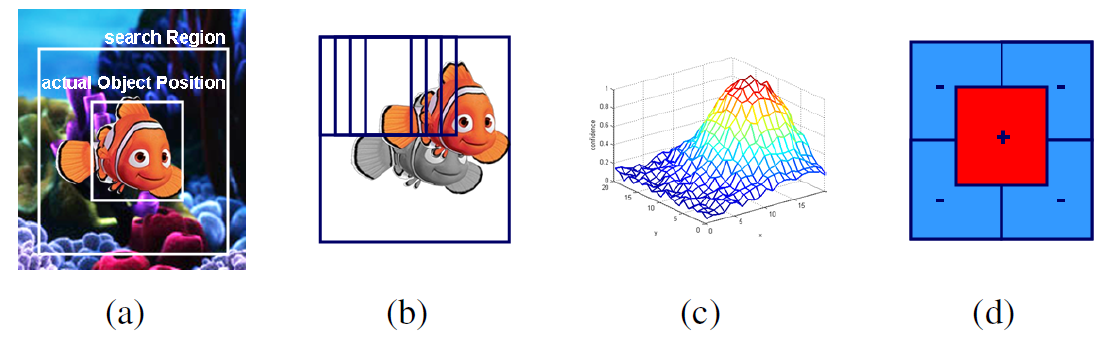
\includegraphics[width=0.7\linewidth]{../resources/img/grundlagen/tracking}
    \caption[Übersicht Tracking mit Klassifikator]{Übersicht Tracking mit Klassifikator \cite[]{Grabner}}
    \label{fig:grund_tracking}
\end{figure}

Das Erlernen eines stabilen Klassifikators in der ``Tracker-Application'' basiert auf der Arbeit
\textit{``Real-Time Tracking via On-line Boosting''} von \cite[]{Grabner}.
Die Autoren verwenden einen On-line AdaBoost Algorithmus, welcher mehrere \textit{schwache}
Klassifikatoren zu einem \textit{starken} Klassifikator kombiniert.
Schwache Klassifikatoren müssen hierbei nur eine Erkennungsrate von mehr als 50\% besitzen und somit
wenig besser als zufallsbedingtes Auswählen sein.
Starke Klassifikatoren entstehen durch die Kombination von mehreren schwachen Klassifikatoren.
Die Auswahl von schwachen Klassifikatoren erfolgt über sogenante Selektoren, welche aus einer Menge
immer jenen wählen, welcher die geringste Fehlerrate bei der Erkennung
der Trainings-Objekte besitzen. Der Klassifikator mit der schlechtesten Erkennungsrate wird in jeder
Trainingsiteration ersetzt, um das Training zu verbessern.
Großer Vorteil der On-line AdaBoost Methode ist, dass sie es ermöglicht, starke Klassifikatoren während des
eigentlichen Trackingvorganges zu erlernen. Nach jedem Trackingschritt wird das erfolgreich erkannte
Objekt in Trainingssätze zerlegt, auf welche die Klassifikatoren angewandt werden um ihre Performance zu evaluieren.
So wird in jedem Schritt die Menge der schwachen Klassifikatoren und der Selektoren aktualisiert. Die Wahl
von effizient berechenbaren schwachen Klassifikatoren macht dies möglich.

Die in \cite[]{Grabner} und der ``Tracker-Application'' verwendeten Klassifikatoren sind binär, das heißt,
sie teilen Objekte in die zwei Klassen \textit{erkannt} und \textit{nicht erkannt} auf.
Konkret werden Haar-ähnliche Bildmerkmale nach \cite[]{Viola} als schwache Klassifikatoren verwendet.
Diese sind ein Mittel zur Identifikation von Kontrastunterschieden in Bildern, welche sich sehr gut
zur Erkennung von Kanten und Linien eigenen. Ein Beispiel der Haar-ähnlichen Merkmale und ihres Einsatzes
bei der Gesichtserkennung ist in Abbildung \ref{fig:grund_hair_like} dargestellt.

Diese Merkmale werden als schwache Klassifikatoren mit zufälliger Skalierung, Größe und Position
auf dem Bild platziert. Sie suchen in dieser Region anschließend nach den von dem Muster definierten
Konturunterschieden. Eine Bereich gilt als erkannt, wenn der Betrag der Differenz der Pixelsumme des weißen und
schwarzen Bereiches des Musters unter einem festgelegten Grenzwert liegt.

\begin{figure}[H]
    \centering
    \subfloat[]{{
        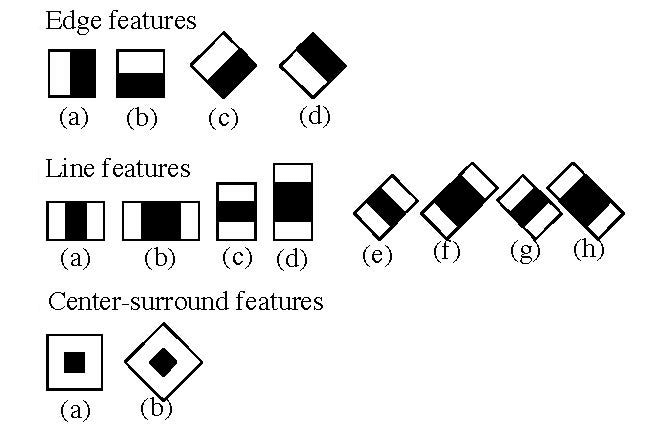
\includegraphics[width=0.4\linewidth]{../resources/img/grundlagen/hair_like_features}
    }}
    \qquad
    \subfloat[]{{
        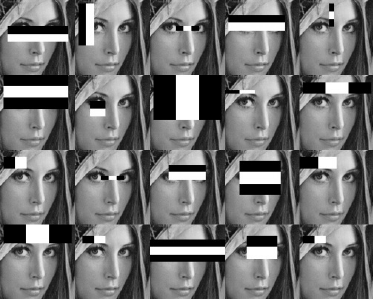
\includegraphics[width=0.35\linewidth]{../resources/img/grundlagen/hair_like_features_2}
    }}
    \caption[a) Haar-ähnliche Merkmale b) Beispiele für erkannte Regionen in einem Gesicht]{a) Haar-ähnliche Merkmale b) Beispiele für erkannte Regionen in einem Gesicht \cite[]{DivyanshDwivedi2018}}
    \label{fig:grund_hair_like}
\end{figure}

\section{Datenaufbereitung und Bereinigung}
\label{sec:tra_preprocessing}

% ALLGEMEINE Beschreibung von möglichen Datenbereinigungsschritten
% Resampling (Distanz oder Geschwindigkeit)
% Padding etc. (Interpolation)
% Glättung (RANSAC, Wavelet)

\section{Clusteranalyse}
\label{sec:tra_clustering}

Die Clusteranalyse (kurz Clustering) ist ein wichtiges Werkzeug zur Auswertung von Daten unterschiedlichster
Art. Sie stellt dabei kein konkretes Vorgehen oder einen Algorithmus dar, sondern beschreibt ein
allgemeines Problem, welches auf unterschiedlichste Weise gelöst werden kann.
Grundsätzlich ist das Ziel der Clusteranalyse, Datenobjekte aufgrund ihrer Eigenschaften und Beziehungen
untereinander so zu gruppieren, dass sich die Objekte einer Gruppe möglichst stark ähneln und sich
von den Objekten anderer Gruppen möglichst stark unterscheiden. Je höher die \textit{Homogenität} in einem Cluster
und die \textit{Differenz} zwischen den Clustern, desto besser ist die gewählte Clustering Methode.
Der Einsatz von Clustering ist in vielen Anwendungsgebieten und in den unterschiedlichsten wissenschaftlichen
Disziplinen sehr beliebt, um ein Verständnis für Daten zu erhalten beziehungsweise diese verarbeiten zu können.
So kommt die Clusteranalyse unter anderem in den Feldern des maschinellen Lernens, der Mustererkennung, Bildanalyse,
der Biologie (Taxonomie) oder im Bereich Data Mining zum Einsatz. \cite[]{tan2007introduction}

Die Clusteranalyse hat viel mit dem Problem der Klassifizierung von Daten gemein, insofern sie Datenobjekten
Label zuordnet. Im Gegensatz zu \textit{überwachten} Klassifizierungsansätzen, wie dem heute populären überwachten
Lernen, leiten Cluster-Algorithmen die Label allerdings alleine aus den vorhandenen Daten ab.
Es kommen keine Vergleichsobjekte mit bekannten, händisch vergebenen Labeln zum Einsatz.
Aus diesem Grund wird die Clusteranalyse auch häufig als \textit{unüberwachte Klassifizierung} bezeichnet. \cite[]{tan2007introduction} 

Das Konzept eines \textit{Clusters} ist nicht genau definiert, was in einer Vielzahl an unterschiedlichen Ansichten
und Algorithmen resultiert, welche sich jeweils für andere Anwendungsfälle eignen und verschiedene Eigenschaften
besitzen. Hieraus ergibt sich auch die Tatsache, dass Clustering keine selbsttätiger Prozess ist, welcher sich auf
einheitliche Weise auf unterschiedliche Probleme anwenden lässt. Jedes Problem erfordert die individuelle und sorgfältige
Auswahl eines passenden Algorithmus, eines Distanzmaßes und der richtigen Parameter. Die Bestimmung dieser geschieht
iterativ und nicht selten nach dem Prinzip des \textit{Trial and Error}. In Abbildung \ref{fig:grund_clustering_example}
ist beispielhaft ein Datensatz (links) mit -- für den Menschen intuitiv ersichtlich -- 7 unterschiedlichen Clustern (rechts)
dargestellt. Nach \cite[]{Jain2010} kann kein verfügbarer Clustering Algorithmus diese allerdings alle erkennen.
\cite[]{Jain1999, tan2007introduction}

\begin{figure}[H]
    \centering
    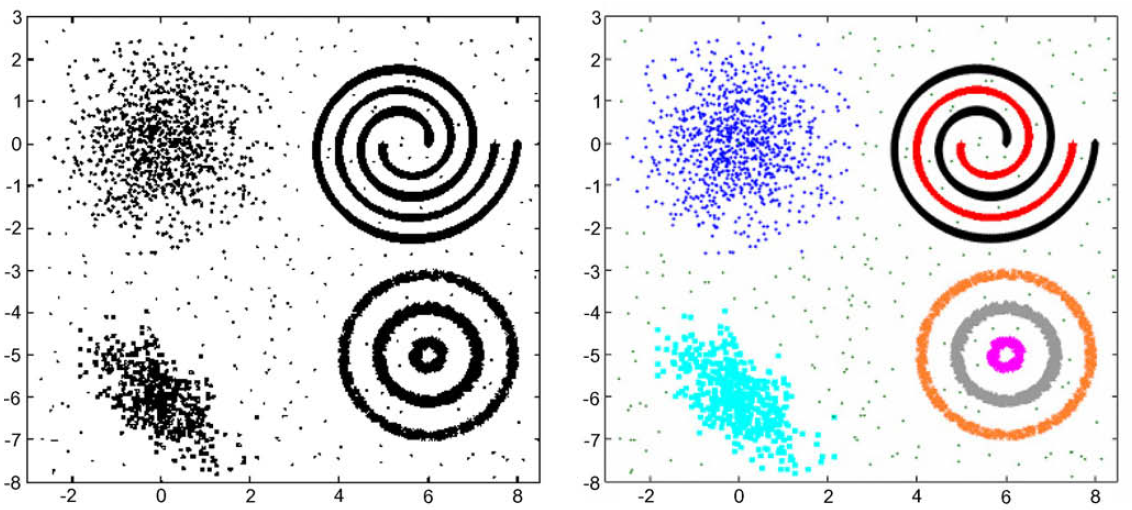
\includegraphics[width=0.8\linewidth]{../resources/img/grundlagen/clustering_example}
    \caption[Rohdaten (links) und erwünschtes Clustering-Ergebnis (rechts)]{Rohdaten (links) und erwünschtes Clustering-Ergebnis (rechts) \cite[]{Jain2010}}
    \label{fig:grund_clustering_example}
\end{figure}

Aufgrund der Limitationen, welche alle Cluster-Algorithmen besitzen, muss der Analyst sich vor deren Anwendung intensiv
mit den zu verarbeitenden Daten beschäftigen. Er muss ein Verständnis dafür besitzen, welche Struktur die Daten
besitzen, beziehungsweise annehmen können, und nach welchen Mustern zu suchen ist.
Besonders wichtiger ist zudem auch die Auswahl der richtigen, das heißt relevanten, Datenmerkmale (\textit{``Feature-Selection''})
und die Wahl deren Repräsentation. Die Selektion und gegebenenfalls Transformation der Daten muss in einem
Vorverarbeitungsschritt geschehen, dessen Qualität einen maßgeblichen Einfluss auf das finale Clustering Ergebnis hat.
Basierend auf dieser Beschreibung und \cite[]{Jain1999}, lässt sich der Ablauf einer Clusteranalyse wie folgt darstellen:

% TODO: Grafik selbst neu erstellen
% (Feature Selection --> Feature Transformation --> Ähnlichkeitsmessung --> Clustering --> Feedback)
\begin{figure}[H]
    \centering
    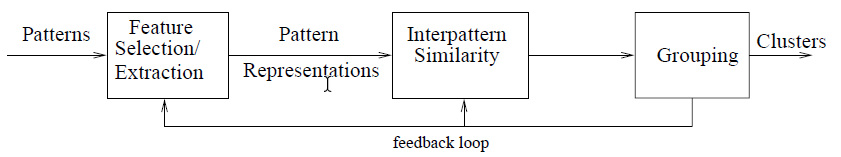
\includegraphics[width=0.8\linewidth]{../resources/img/grundlagen/clustering_workflow}
    \caption{Ablauf einer Clusteranalyse}
    \label{fig:grund_clustering_workflow}
\end{figure}

Einige wichtige Clustering-Ansätze sind die Vernetzungs-Modelle, Centroid-basierte-Modelle, Verteilungs-Modelle
oder Dichte-Modelle. Diese und einige der stellvertretende Algorithmen werden in nachfolgendem Abschnitt \ref{sec:cluster_algos}
beschrieben.

\subsection{Cluster Algorithmen}
\label{sec:cluster_algos}

\subsection{Distanzmaße zum Vergleich von Fahrzeugtrajektorien}
\label{sec:distance_measures}

\section{Untersuchung möglicher Straßentopologien}
\label{sec:street_topologies}